%%%%%%%%%%%%%%%%%%%%%%%%%%%%%%%%%%%%%%%%%%%%%%%%%%%%%%%%%%%%%%%%%%%%%%%%%%%%
%% Author template for INFORMS Journal on Data Science (ijds) [interim solution; new styles under construction]
%% Mirko Janc, Ph.D., INFORMS, mirko.janc@informs.org
%% ver. 0.91, March 2015 - updated November 2020 by Matthew Walls, matthew.walls@informs.org
%% Adapted for rticles by Rob J Hyndman Rob.Hyndman@monash.edu. Dec 2021
%%%%%%%%%%%%%%%%%%%%%%%%%%%%%%%%%%%%%%%%%%%%%%%%%%%%%%%%%%%%%%%%%%%%%%%%%%%%
\documentclass[,,nonblindrev]{informs}

\OneAndAHalfSpacedXI
%%\OneAndAHalfSpacedXII % Current default line spacing
%%\DoubleSpacedXII
%%\DoubleSpacedXI

%% BEGIN MY ADDITIONS %%
\usepackage{hyperref}

% tightlist command for lists without linebreak
\providecommand{\tightlist}{%
  \setlength{\itemsep}{0pt}\setlength{\parskip}{0pt}}



\usepackage{booktabs}
\usepackage{tabularx}
\usepackage{graphicx}
\usepackage{tikz}
\usepackage{siunitx}
\usepackage{tablefootnote}
\usepackage{longtable}
\usepackage{threeparttable}
\usepackage{natbib}
\usepackage{caption}

%% END MY ADDITIONS %%


% Natbib setup for author-year style
\usepackage{natbib}
 \bibpunct[, ]{(}{)}{,}{a}{}{,}%
 \def\bibfont{\small}%
 \def\bibsep{\smallskipamount}%
 \def\bibhang{24pt}%
 \def\newblock{\ }%
 \def\BIBand{and}%


%% Setup of theorem styles. Outcomment only one.
%% Preferred default is the first option.
\TheoremsNumberedThrough     % Preferred (Theorem 1, Lemma 1, Theorem 2)
%\TheoremsNumberedByChapter  % (Theorem 1.1, Lema 1.1, Theorem 1.2)
\ECRepeatTheorems

%% Setup of the equation numbering system. Outcomment only one.
%% Preferred default is the first option.
\EquationsNumberedThrough    % Default: (1), (2), ...
%\EquationsNumberedBySection % (1.1), (1.2), ...

% For new submissions, leave this number blank.
% For revisions, input the manuscript number assigned by the on-line
% system along with a suffix ".Rx" where x is the revision number.
\MANUSCRIPTNO{}

%%%%%%%%%%%%%%%%
\begin{document}
%%%%%%%%%%%%%%%%

% Outcomment only when entries are known. Otherwise leave as is and
%   default values will be used.
%\setcounter{page}{1}
%\VOLUME{00}%
%\NO{0}%
%\MONTH{Xxxxx}% (month or a similar seasonal id)
%\YEAR{0000}% e.g., 2005
%\FIRSTPAGE{000}%
%\LASTPAGE{000}%
%\SHORTYEAR{00}% shortened year (two-digit)
%\ISSUE{0000} %
%\LONGFIRSTPAGE{0001} %
%\DOI{10.1287/xxxx.0000.0000}%

% Author's names for the running heads
% Sample depending on the number of authors;
\RUNAUTHOR{%
Jameson, Saghafian, Huckman
 and Hodgson
}
% \RUNAUTHOR{Jones and Wilson}
% \RUNAUTHOR{Jones, Miller, and Wilson}
% \RUNAUTHOR{Jones et al.} % for four or more authors
% Enter authors following the given pattern:
%\RUNAUTHOR{}

\RUNTITLE{Judicious Batching: The Impact of Batch Ordering Imaging Tests
in the Emergency Department}

\TITLE{Judicious Batching: The Impact of Batch Ordering Imaging Tests in
the Emergency Department}

\ARTICLEAUTHORS{%
\AUTHOR{Jacob Jameson}
\AFF{Interfaculty Initiative in Health Policy, Harvard
University, \EMAIL{\href{mailto:jacobjameson@g.harvard.edu}{\nolinkurl{jacobjameson@g.harvard.edu}}}}

\AUTHOR{Soroush Saghafian}
\AFF{Kennedy School of Government, Harvard
University, \EMAIL{\href{mailto:soroush_saghafian@hks.harvard.edu}{\nolinkurl{soroush\_saghafian@hks.harvard.edu}}}}

\AUTHOR{Robert Huckman}
\AFF{Harvard Business
School, \EMAIL{\href{mailto:rhuckman@hbs.edu}{\nolinkurl{rhuckman@hbs.edu}}}}

\AUTHOR{Nicole Hodgson}
\AFF{Mayo
Clinic, \EMAIL{\href{mailto:Hodgson.Nicole@mayo.edu}{\nolinkurl{Hodgson.Nicole@mayo.edu}}}}

%
}

\ABSTRACT{We use practice variation across physicians to uncover the
role of test-ordering on care delivery in the ED. Using records of over
45,000 Mayo Clinic emergency department visits, we find that
quasi-random assignment to a top (versus bottom) decile batching
physician significantly increases excess diagnostic testing.
Instrumental variable results show that batching leads to an additional
13.5 tests per 100 batches, resulting in excess tests that would not
have been ordered under a sequential-ordering strategy. Contrary to
expectations, batch ordering does not reduce ED length of stay or affect
72-hour return rates, challenging the perceived efficiency of batching
and highlighting the necessity for more targeted testing strategies in
emergency care.}

\KEYWORDS{Emergency Department, Operational Effeciency, Diagnostic
Testing}

\maketitle


\hypertarget{sec:I}{%
\section{Introduction}\label{sec:I}}

Healthcare delivery, particularly in the emergency department (ED), is a
delicate balance that involves ensuring optimal patient outcomes while
optimizing resource utilization. Achieving these twin goals requires
timely and accurate diagnosis, which in turn enables prompt and
appropriate treatment, consequently improving patient prognosis and
reducing the likelihood of adverse events. Furthermore, efficient
patient discharge from the ED can help alleviate overcrowding, a severe
issue with potential consequences including higher complication rates
and increased mortality \citet{bernstein2009}.

One important factor that can impact the speed and effectiveness of
diagnosis in the ED is the availability and performance of diagnostic
tests \citet{naseim2015}. A variety of diagnostic tests are used in the
ED, including laboratory tests, imaging studies, and specialized tests.
These tests can provide valuable information about a patient's condition
and help to guide treatment decisions.

A critical question in this context pertains to whether physicians in
the ED should batch order diagnostic tests or order them sequentially.
This decision essentially represents a tradeoff between reducing patient
length of stay and risk of over-testing. Over-testing, or performing
unnecessary tests, can lead to increased costs, unnecessary patient
anxiety, and potential harm from follow-up of false-positive results
\citet{koch2018}. Conversely, keeping a patient for an extended time to
perform all possible tests could lead to ED overcrowding, an issue
associated with severe consequences, as mentioned earlier. Instead, what
is needed is a reasonable balance between the number of diagnostic tests
performed and the total time the patient is kept in the ED before either
being admitted or discharged. Several studies have demonstrated that
optimizing the ED patient flow process can result in significant
improvements \citet{saghafian2015}, however, research surrounding test
ordering strategies to improve the patient flow processes remains
limited.

In this paper, we use data from over 45,000 patient visits to the ED
that occur during our study period to quantify the benefits and
consequences of batching versus sequentially ordering diagnostic tests
on patient length of stay, re-admission, and resource utilization. Our
empirical strategy exploits random assignment of patients to ED
physicians who differ in their propensity to batch-order diagnostic
tests. When patients arrive at the ED, they are assigned to a physician
based on availability, with no discretion on either side. Thus, patients
who arrive at the ED at similar times are randomly assigned to
physicians who vary in their willingness to batch order diagnostic
tests. We measure physician tendency to batch using a leave-out,
residualized measure based on all other patients the physician has seen
in the ED in the study period. The tendency measure strongly predicts
the ED test batch outcome but is uncorrelated with patient and ED visit
characteristics.

We start by evaluating the reduced-form effects of ED provider
batch-ordering tendency on downstream patient outcomes and turnaround
time. We find that practice variation as captured by physician
batch-ordering tendency has large and significant consequences. Being
treated by a provider in the top decile of the tendency distribution,
compared to being treated by someone in the bottom decile results in an
additional 2 diagnostic test per 100 patient encounters after
controlling for the physician's underlying propensity to test.

Physician care takes on multiple dimensions besides the decision to
batch order diagnostic tests. Employing a placebo exercise, we find
evidence that that excess testing occurs after having seen a
high-batching physician is due to batching from this physician, as
opposed to other differences across physician in care that correlate
with batching tendency: we find no effects of physician batch tendency
on key outcomes for a ``placebo sample'' of patients who visit the ED
for conditions that rarely result in batched orders.

With the caveat that other unobserved dimensions of physician care may
impact patient outcomes, we employ physician batch tendency as an
instrumental variable for having tests batch ordered in the ED to
quantify the effect of batching directly. Because of the institutional
features of the ED, our research design closely approximates an RCT that
assigns patients to batch-ordering or sequential-ordering arm. In the
ED, patients have no discretion over choosing providers, and in our
specific ED, physicians have discretion over choosing patients,
alleviating major selection issues present in other health care
settings. Furthermore, physicians exhibit wide variation in practice
behavior in batch-ordering, even within the same hospital, while
following the same guidelines. Finally, patient-physician interactions
in the ED are typically well documented, short, and one-off,
constraining physician decision-making to a more limited,
better-observed choice set than present in settings such as specialty or
primary care.

In sum, exploiting practice variation in ED settings shuts down other
(but not all) potential channels besides test batching that are present
in other settings, determine length of stay, and impact patient
outcomes. This approach allows us to move closer to identifying the
causal impact of batch-ordering diagnostic tests on patient outcomes and
resource utilization. It is important to note that this paper studies
the impact of batch-ordering through a batching decision requiring
clinical judgment (within practice norms) rather than through specific
hospital policies, differences in adherence to clinical practice
guidelines, or substandard care.

The remainder of this paper is structured as follows. The next section
describes the data source and outlines our baseline sample. The
empirical strategy and its accompanying identifying assumptions are laid
out in Section III. Section IV presents the results. Section V draws
implications for batch-ordering policies. The last section concludes.

\hypertarget{sec:II}{%
\section{Data and Definitions}\label{sec:II}}

Our study was conducted in the Emergency Department (ED) of the Mayo
Clinic of Arizona, a tertiary care hospital without obstetrical
services, an inpatient pediatrics unit, or a trauma designation. During
the study period, the ED recorded approximately 43,000 visits per year,
managed across 26 treatment rooms and up to 9 hallway spaces. The
department is exclusively staffed by board-eligible or board-certified
emergency physicians (EPs), with rotating residents overseeing about
10\% of patient volume. Physicians operate in a unique workflow that
includes staggered 8.5-hour shifts and a rotational patient assignment
system, minimizing potential selection bias in patient encounters.

We conducted a retrospective review of comprehensive ED operational data
from 10/6/2018 through 12/31/2019, coinciding with the initiation of a
new electronic medical record. The dataset includes detailed patient
demographics, chief complaints, vital signs, emergency severity index
(ESI), length of stay (LOS), and resource utilization metrics. This
period was chosen to provide a robust data set while excluding the
influence of the coronavirus pandemic.

\hypertarget{sample-construction}{%
\subsection{Sample Construction}\label{sample-construction}}

Our research design focuses on adults who visit the Mayo Clinic of
Arizona ED. We observe approximately \(48,000\) such visits during the
study period. To improve power, we drop encounters with rare chief
complaints (\(<1000\) total encounters of this kind) and complaints
where a batch order occurs less than \(2\) percent of the time. Since
batch orders are rare for these cases, our physician batch tendency
instrument could suffer from a weak instrument problem if we included
them. Examples of complaints dropped include Upper Respiratory Symptoms
and Urinary Complaints. Excluding these conditions does not introduce
selection bias unless physician test batching tendency is orthogonal to
physician diagnosing behavior. While this assumption may be violated if
we were to use a very detailed level of chief complaint information upon
which to base our exclusion criterion, it is plausibly satisfied when
using broad complaint categories. In order to estimate a precise measure
of physician-level batch tendency, we further restrict our sample to the
\(36,765\) encounters involving full-time physicians who treat over 500
ED cases per year.

\hypertarget{variable-definitions}{%
\subsection{Variable Definitions}\label{variable-definitions}}

Our explanatory variable in the IV analysis, \(Batched_i\), is an
indicator for whether patient \(i\) has their tests batch-ordered at
their ED encounter. While the patient could decide not to undergo the
tests ordered by the physician, this is rare in practice. Below, we
detail our primary outcomes: (a) ED length of stay (LOS), and (b)
resource utilization.

\emph{(a) ED length of stay (LOS).}-- ED-LOS is a critical measure of
efficiency and patient throughput in emergency care settings. It is
defined as the duration from a patient's arrival to the ED until their
departure, whether by discharge or admission to the hospital. The
hypothesis is that batch testing may lead to shorter ED-LOS, potentially
improving patient throughput and reducing crowding.

\emph{(b) Resource Utilization}-- Resource utilization in the ED
typically refers to the extent of medical services and interventions a
patient receives. In this study, we quantify resource utilization by the
total number of distinct diagnostic tests ordered per patient during
their ED stay. This encompasses both initial and subsequent tests. The
hypothesis is that batch testing may lead to variations in the number of
tests ordered, potentially influencing the overall healthcare
expenditure and efficiency.

\emph{(c) 72 Hour Return with Admission}-- This is a binary variable
indicating whether the patient returns to the ED within 72 hours of
their initial visit and is admitted to the hospital. This outcome is
used to assess the quality of care provided during the initial ED visit.
The hypothesis is that batch testing may lead to variations in the
quality of care provided, potentially influencing the likelihood of a
return visit.

\hypertarget{batching}{%
\subsubsection{Batching}\label{batching}}

We define ``batching'' in line with standard emergency medicine
practices. Batching occurs when a physician simultaneously orders a
comprehensive set of diagnostic tests, typically covering a broad range
of potential diagnoses. This contrasts with sequential ordering, where
tests are ordered sequentially based on the information obtained from
each test as needed.

We operationalize batching as occurring when multiple diagnostic imaging
tests are ordered within a 5-minute window. In Section 4.4, sensitivity
analyses on this cutoff point showed that our results are robust to this
definition. Each imaging test (e.g., X-ray, CT scan, Ultrasound) is
considered a separate, distinct test for our study. Therefore, a batch
in our study consists of two or more distinct imaging tests.

\hypertarget{summary-statistics}{%
\subsection{Summary Statistics}\label{summary-statistics}}

hyperref{[}tab{]}\{Table 1\} provides a concise overview of emergency
department (ED) characteristics, patient demographics, and medical tests
based on our study data. The ED maintains an average volume of 24.3
patients, reflecting a significant yet manageable workload. Key
physiological indicators include tachycardia (18.8\%) and tachypnea
(9.51\%), showcasing the critical conditions often treated in emergency
settings. Additionally, fever and hypotension are observed in 2.43\% and
1.57\% of patients, respectively, highlighting the variety of urgent
care demands.

Patient complaints commonly involve abdominal issues (16.9\%), extremity
problems (14.3\%), and chest pain (9.58\%), along with neurological
(9.50\%) and gastrointestinal complaints (9.04\%). These figures
emphasize the frequent health concerns that drive ED visits and the
resources needed for effective response.

The patient demographic profile shows an average age of 58.3 years,
predominantly middle-aged and elderly individuals. Racial distribution
is mainly White (88.6\%), with smaller percentages of Black (4.12\%) and
Asian (2.97\%) populations. A slight majority of patients are female
(54.5\%), indicating gender trends in healthcare utilization.

Diagnostic procedures heavily rely on lab tests (78.5\%), essential for
thorough patient evaluations. Imaging tests such as X-rays (48.1\%) and
CT scans---both non-contrast (23.1\%) and contrast (20.5\%)---play
pivotal roles in diagnostics. The use of ultrasounds (12.5\%) and the
strategy of batch ordering tests (6.32\%) are critical operational
aspects of the ED, reflecting approaches to efficient patient
management.

\begin{table}[ht]
\centering
\caption{Summary Statistics of Emergency Department Encounters}
\label{tab:summary_statistics}
\begin{tabular}{p{10.5cm}cccc}
\toprule
\textbf{} & \textbf{Mean} & \textbf{Q1} & \textbf{Median} & \textbf{Q3} \\
\midrule
\multicolumn{5}{l}{\textbf{Emergency Department Characteristics}} \\
Patients in ED & 24.3 & 16 & 25 & 33 \\
\\
Tachycardic & 0.188 & & & \\
Tachypneic & 0.095 & & & \\
Febrile & 0.024 & & & \\
Hypotensive & 0.016 & & & \\
\\
ESI & 2.74 & 2 & 3 & 3 \\
\\
Complaint: Abdominal Complaints & 0.169 & & & \\
Complaint: Extremity Complaints & 0.143 & & & \\
Complaint: Chest Pain & 0.096 & & & \\
Complaint: Neurological Issue & 0.095 & & & \\
Complaint: Gastrointestinal Issues & 0.090 & & & \\
\midrule
\multicolumn{5}{l}{\textbf{Patient Characteristics}} \\
Arrival Age & 58.3 & 44 & 61 & 75 \\
\\
Race: White & 0.886 & & & \\
Race: Black & 0.041 & & & \\
Race: Asian & 0.030 & & & \\
\\
Gender: Female & 0.545 & & & \\
\midrule
\multicolumn{5}{l}{\textbf{Tests}} \\
X-Ray & 0.481 & & & \\
Ultrasound & 0.125 & & & \\
Non-Contrast CT & 0.231 & & & \\
Contrast CT & 0.205 & & & \\
Lab & 0.785 & & & \\
\\
Imaging Tests were Batch Ordered & 0.063 & & & \\
\bottomrule
\end{tabular}
\begin{tablenotes}
\small
\item \textit{This table reports summary statistics for the baseline sample of emergency department visits during the study period described in the text. Vital signs were categorized as follows: tachycardia (pulse more significant than $100$), tachypnea (respiratory rate greater than $20$), fever (temperature greater than $38^\circ C$), and hypotension (systolic blood pressure less than $90$).}
\end{tablenotes}
\end{table}

\hypertarget{sec:3}{%
\section{Empirical Strategy}\label{sec:3}}

Our empirical strategy closely follows the literature that relies on
quasi-random assignment of agents to cases, often referred to as the
``judges design.'' Papers in this literature typically exploit variation
in the sentencing leniency of judges who work in the same court.
Similarly, we explore batching variation across physicians who work in
the same emergency department. In its reduced form, under the assumption
of quasi-random assignment, this approach allows researchers to identify
the causal effect of being assigned to different types of physicians.
Under additional assumptions, an instrumental variable approach
identifies the causal effect of a given medical decision. We employ both
approaches and lay out their details in the next subsections.

\hypertarget{institutional-details-on-patient-physician-assignment}{%
\subsection{Institutional Details on Patient-Physician
Assignment}\label{institutional-details-on-patient-physician-assignment}}

Contrary to most healthcare settings where patients exhibit choice, they
are predominantly passive in their physician assignment in the ED. In
most EDs, however, physicians have discretion in picking their patients.
In contrast, patients arriving at the Mayo Clinic ED are randomly
assigned to physicians via a rotational patient assignment algorithm
\citet{traub2016emergency}, which removes potential selection bias
concerns for our analyses. In essence, barring arrival time and
shift-level variation, the physician-to-patient matching can be deemed
random. Table \ref{tab:wald_test} displays that patient encounters
(regarding chief complaints and emergency severity) are equitably
distributed across physicians within our study's cohort.

\begin{table}[htbp]
    \centering
    \caption{Balancing Test: Wald Test for Equality of Means}
    \label{tab:wald_test}
    \begin{tabular}{p{10cm}cccc}
        \toprule
        Chief Complaints & Frequency & F-Statistic & $Pr(> F)$ \\
        \midrule
        Abdominal Complaints & 6232 & 2.587 & 0.108 \\ 
        Back or Flank Pain & 2552 & 1.637 & 0.201 \\ 
        Chest Pain & 3525 & 0.407 & 0.524 \\ 
        Extremity Complaints & 5265 & 1.847 & 0.174 \\ 
        Falls, Motor Vehicle Crashes, Assaults, and Trauma & 2381 & 0.023 & 0.880 \\ 
        Gastrointestinal Issues & 3323 & 0.105 & 0.746 \\ 
        Neurological Issue & 3495 & 0.135 & 0.713 \\ 
        Shortness of Breath & 2966 & 1.324 & 0.250 \\ 
        Skin Complaints & 2178 & 0.383 & 0.536 \\ 
        Upper Respiratory Symptoms & 1917 & 0.017 & 0.896 \\ 
        \midrule
        Emergency Severity & Frequency & F-Statistic & $Pr(> F)$ \\
        \midrule
        ESI 1 or 2 & 13914 & 0.011 & 0.915 \\ 
        ESI 3, 4, or 5 & 29386 & 0.010 & 0.921 \\ 
        \bottomrule
    \end{tabular}
\begin{tablenotes}
\small
\item \textit{Table \ref{tab:wald_test} reports the results of a Wald test which was conducted to assess the balance of chief complaints across providers in our dataset. A balanced distribution implies that complaints and severity are evenly distributed across providers, which we expect to be the case due to randomization. The Wald F-statistic and p-value are reported. Robust standard errors (type HC1) were used to account for potential heteroscedasticity in the data.}
\end{tablenotes}
\end{table}

\hypertarget{batch-tendency-construction}{%
\subsection{Batch Tendency
Construction}\label{batch-tendency-construction}}

To measure physician batch tendency, we use the physician's residualized
leave-out average batch rate. This measure is derived from two steps
following the approaches taken by \citet{doyle2015measuring},
\citet{dobbie2018effects}, and \citet{eichmeyer2022pathways}. First, we
obtain residuals from a regression model, which includes all ED
encounters in our sample period.

\begin{equation}
Batched_{i,t} = \alpha_0 + \alpha_{ym} + \alpha_{dt} + \alpha_{complaint\_esi} + \alpha_{lab} + \varepsilon_{i,t}
\end{equation}

Where \(Batched_{i,t}\) is a dummy variable equal to one if patient
\(i\) had their imaging tests batch ordered on encounter that took place
on date \(t\). Fixed effects include year-month fixed effects,
\(\alpha_{ym}\), to control for time and seasonal variation in batching,
such as hospital-specific policies (e.g.~initiatives to eliminate excess
testing) or seasonality in ED visits. We also control for
``shift-level'' variations that include both physician scheduling and
patient arrival with day of week-time of day fixed effects,
\(\alpha_{dt}\). Chief complaint by severity fixed effects,
\(\alpha_{complaint}\), were also included to increase precision.
Finally, a binary variable for whether or not laboratory tests were
ordered, \(\alpha_{lab}\), was included to account for the complexity of
the case. As stated earlier, these controls are more than what is
required for our quasi-random assignment assumption. Under the
assumption that we have captured the observables under which
quasi-random assignment occurs in the ED, the unexplained variation--
the physician's contribution-- resides in the error term,
\(\varepsilon_{i,t}\).

In step two, the tendency measure for patient \(i\) seen by physician
\(j\) is computed as the average residual across all other patients seen
by the physician that year:

\begin{equation}
Tendency_{i,j}^{phys} =
\frac{1}{N_{-i,j}} \sum_{i' \in \{J \backslash i\}}\hat{\varepsilon}_{i'}
\end{equation}

where \(\hat{\varepsilon}_{i'} = \hat{Batch}_{i'} - Batch_{i'}\) is the
residual from equation (1); \(J\) is the set of all ED encounters
treated by physician \(j\); and \(N_{-i,j} = |\{J \backslash i\}|\), the
number of cases that physician has seen that year, excluding patient
\(i\). This leave-out mean eliminates the mechanical bias that stems
from patient \(i\)'s own case entering into the instrument. The measure
is interpreted as the average (leave-out) batch rate of patient \(i\)'s
physician, relative to other physicians in that hospital-year-month,
hospital-day of week-time of day.

We document that the Mayo Clinic ED physicians exhibit wide, systematic
variation in their propensity to batch order diagnostic tests. Figure
\ref{fig:physician_batching} graphs the frequency with which physicians
batch order across different chief complaints, highlighting that the
variation in batching differs starkly. We note that there is high
correlation between

\begin{figure}[h]
  \centering
  \caption{Variation in Physician Batching}
  \label{fig:physician_batching}
  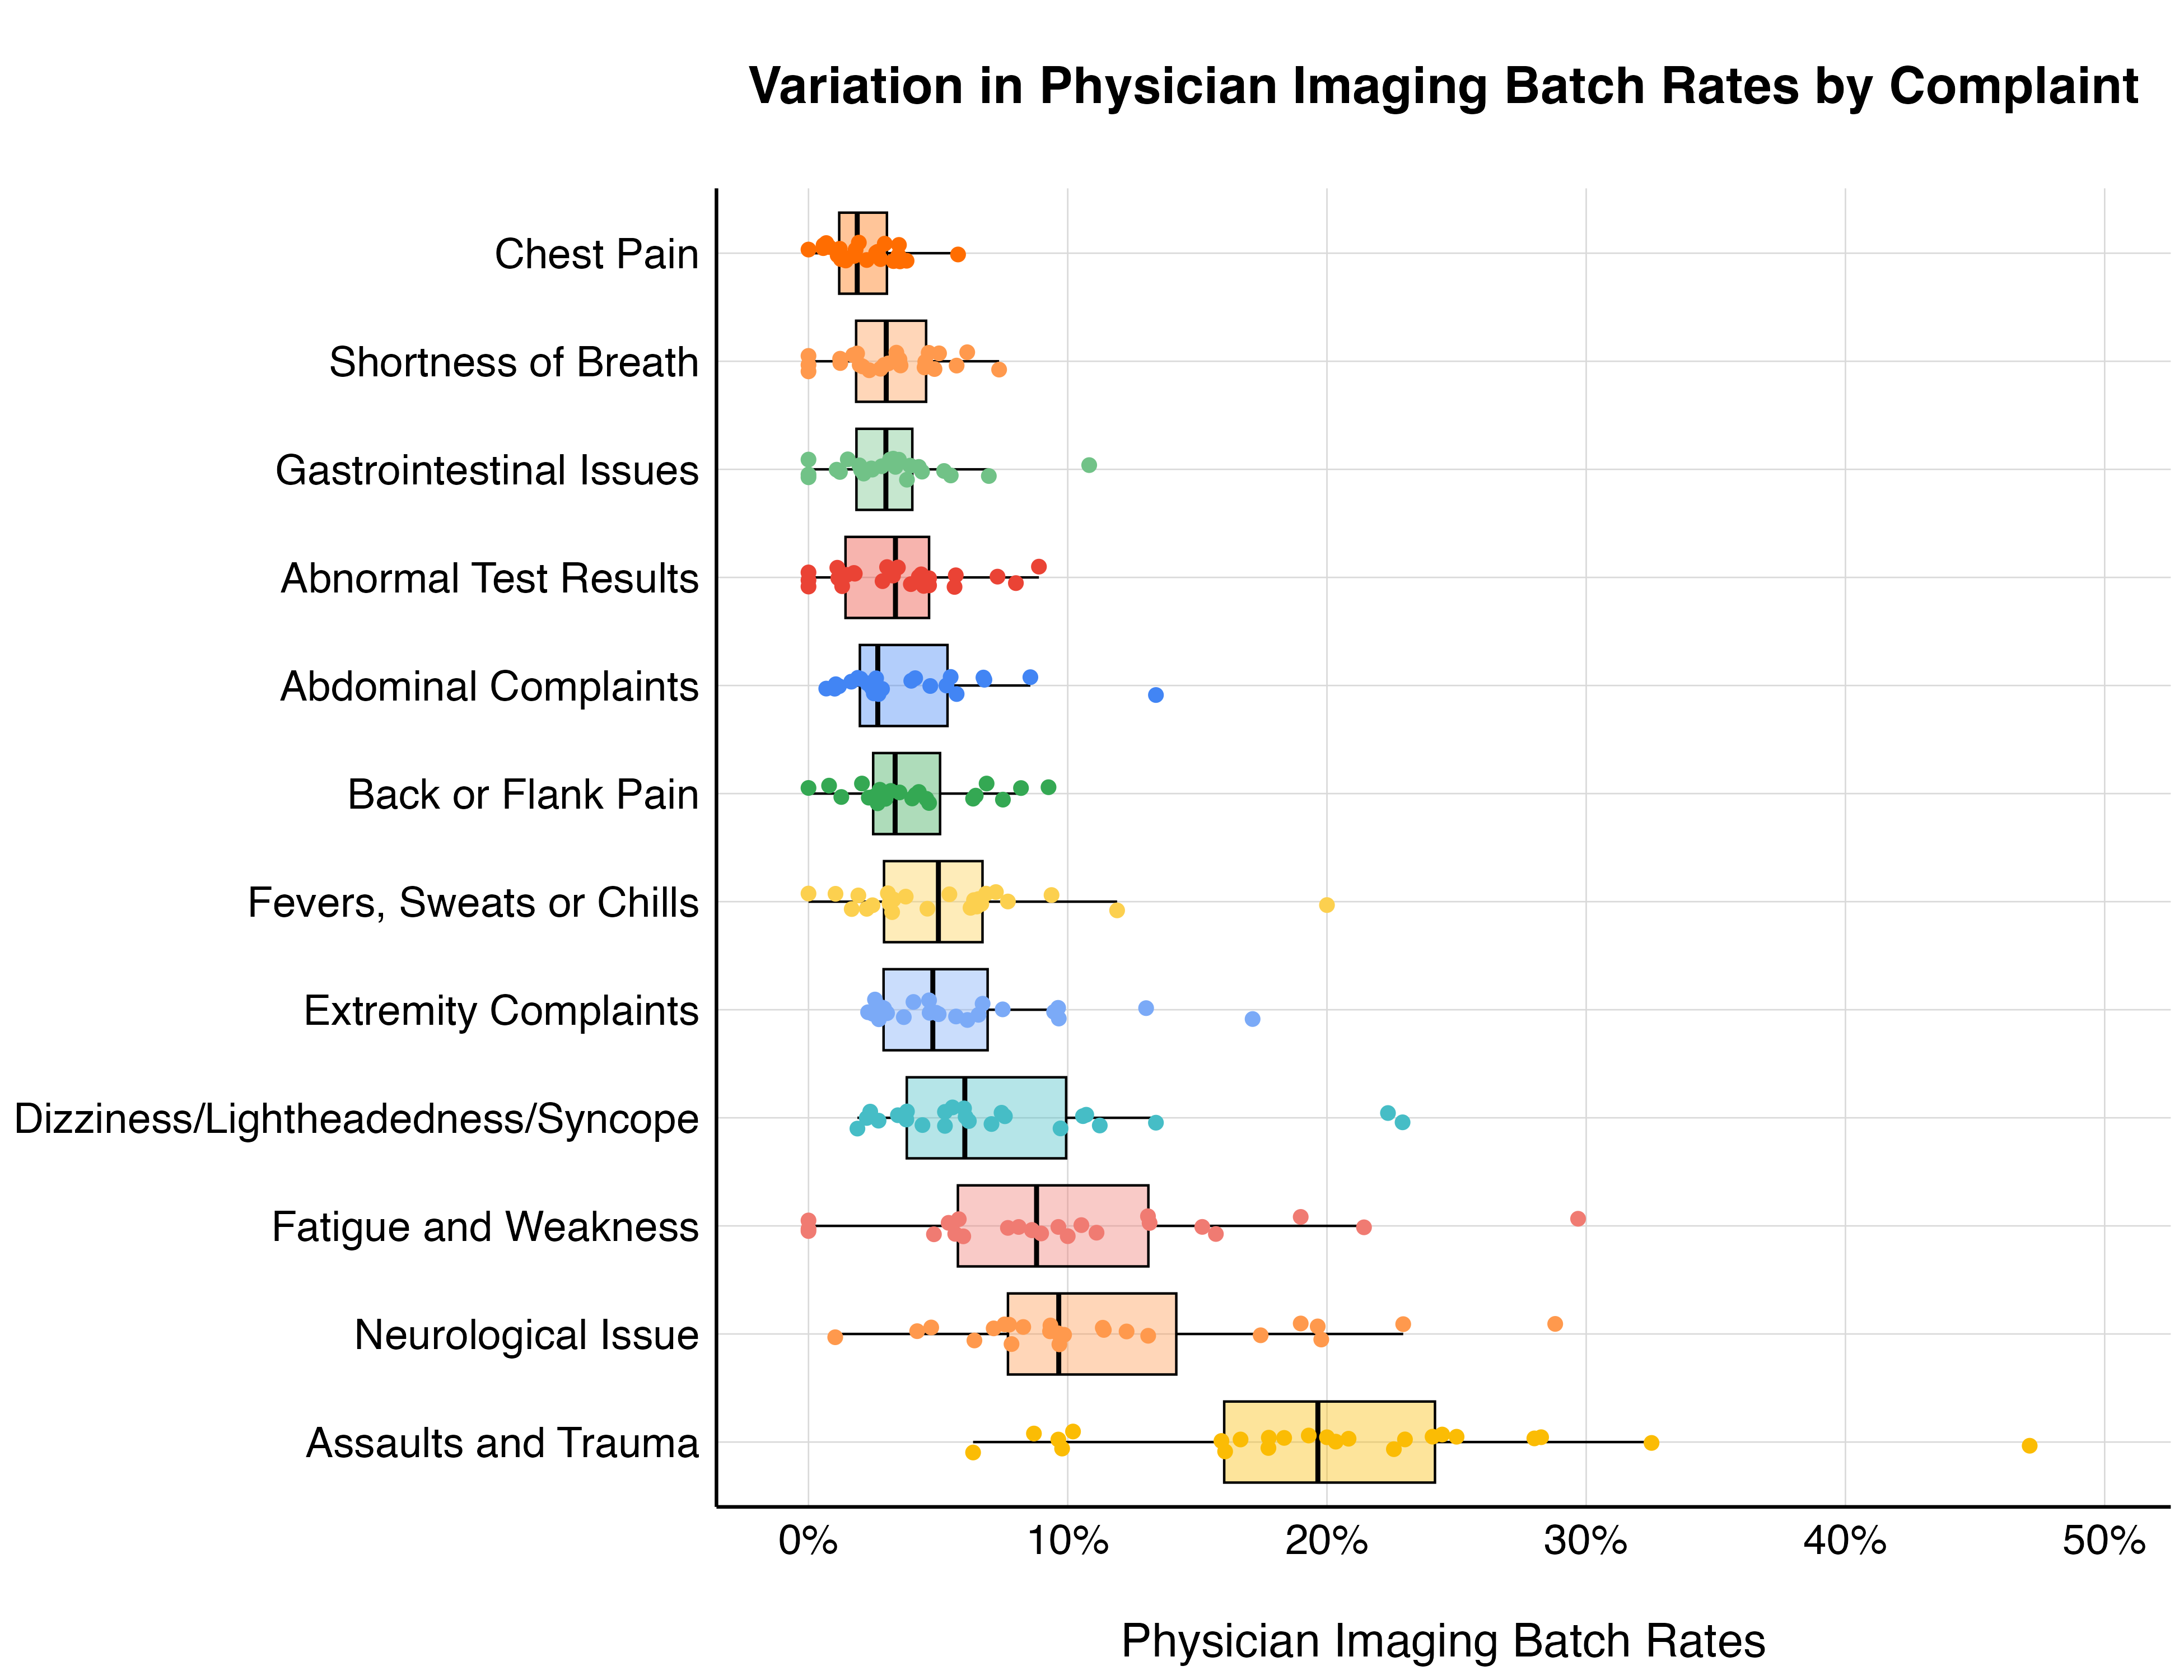
\includegraphics[width=4.25in]{../outputs/figures/Figure 1.png}
\begin{tablenotes}
\small
\item \textit{Figure \ref{fig:physician_batching} illuminates the marked differences among physicians in their propensity to batch-order diagnostic tests.}
\end{tablenotes}  
\end{figure}

\hyperref[table:first_stage]{Table 1} illustrates the ``first stage''
results from both linear and probit models, emphasizing the robust
relevance of the instrument across different statistical frameworks. In
both modeling approaches, a 10 percentage point increase in the
batch-tendency of physicians consistently results in a significant
increase in the likelihood of batch ordering tests in the emergency
department---1.15 percentage points in the linear model and 93.24
percentage points in the probit model. This consistent significance
across models underscores the strength and validity of the
batch-tendency as an instrumental variable, confirming its utility in
controlling for unobserved confounders and providing a reliable basis
for further causal inference. Clustering standard errors at the provider
level ensures robust inference, reinforcing the instrument's credibility
irrespective of the analytical method employed.

\begin{table}[!htbp] \centering 
  \caption{Comparison of First Stage Estimates: Linear vs. Probit Models}
  \label{table:first_stage}
\begin{tabular}{@{\extracolsep{5pt}}lcccccc} 
\\[-1.8ex]\hline 
\hline \\[-1.8ex] 
 & \multicolumn{3}{c}{Linear Model} & \multicolumn{3}{c}{Probit Model} \\ 
\cline{2-4} \cline{5-7}
\\[-1.8ex] & (1) & (2) & (3) & (1) & (2) & (3)\\ 
\hline \\[-1.8ex] 
 Batch Tendency & 1.25$^{***}$ & 1.24$^{***}$ & 1.15$^{***}$ & 8.657$^{***}$ & 9.135$^{***}$ & 8.515$^{***}$ \\ 
  & (0.04) & (0.03) & (0.02) & (0.659) & (0.709) & (0.789) \\ 
  & & & & & & \\
\textit{Day of Week-Time of Day FE} & $\checkmark$ & $\checkmark$ & $\checkmark$ & $\checkmark$ & $\checkmark$ & $\checkmark$ \\
\textit{Month of Year FE} & $\checkmark$ & $\checkmark$ & $\checkmark$ & $\checkmark$ & $\checkmark$ & $\checkmark$ \\
\textit{Complaint/Severity FE} & & $\checkmark$ & $\checkmark$ & & $\checkmark$ & $\checkmark$ \\
\textit{Laboratory Tests Ordered} & & & $\checkmark$ & & & $\checkmark$ \\
\hline 
\hline \\[-1.8ex] 
F Statistic & 13.13 & 26.02 & 29.38 &  &  &  \\
Akaike Inf. Crit. & & & & 16,957.210 & 15,657.200 & 15,349.280 \\ 
\\
\textit{N} & 36,765 & 36,765 & 36,765 & 36,765 & 36,765 & 36,765 \\ 

\hline \\[-1.8ex] 
\end{tabular} 
\begin{tablenotes}
\small
\item \textit{Estimates of the first stage for the baseline sample described in the text. Seasonality shift fixed effects include Year-Month and Hospital-Day of week-Hour of day fixed effects. Chief complaint comes from the cleaned complaint that the patient came in with at the initial encounter. Column 3 corresponds to the baseline controls. Robust standard errors are clustered at the physician level.}
\item $*** p < 0.001$, $** p < 0.01$, $* p < 0.05$.
\end{tablenotes}
\end{table}

To estimate the reduced-form effects of being treated by a
batch-preferring physician, we estimate the following equation:

\begin{equation}
Y_i = \mu_0 + \mu_1 Tendency_{i,j}^{phys} + \gamma X_i + \nu_i
\end{equation}

This reduced form will allow us to check that our instrument is a strong
instrument. To study the effects of test batching in the ED on an
outcome \(Y_i\), we estimate the following 2SLS equations using our
baseline sample:

\begin{equation}
Y_i = \beta_0 + \beta_1 Batched_i + \theta X_i + \varepsilon_i
\end{equation}

\begin{equation}
Batched_i = \delta_0 + \delta_1 Tendency_{i,j}^{phys} + \delta_2 X_i + \nu_i
\end{equation}

Where \(Y_i\) represents our main outcomes of interest: length of stay,
72 hour readmission, and resource utilization. and \(X_i\) is the same
as in the reduced-form approach. \(Batched_i\) variable suffers from
potential endogeneity concerns. For example, injury severity may be
unobserved and correlated with need to run multiple tests, which in turn
also affects length of stay. Hence, we instrument \(Batched_i\) with the
assigned physician \(j\)'s underlying tendency to batch,
\(Tendency_{i,j}^{phys}\). We cluster robust standard errors at the
physician level to account for the assignment process of patients to
physicians.

\hypertarget{identifying-assumptions}{%
\subsection{Identifying Assumptions}\label{identifying-assumptions}}

The reduced-form approach delivers an unbiased estimate of the causal
effect of being treated by a higher tendency to batch physician, since
assignment of patients to ED physicians is random, conditional on
seasonality and shift (``conditional independence''). The
residualization in equation (1) controls for more controls than required
to achieve quasi-random assignment; they are included for statistical
precision in measuring physician tendency to batch.

Our instrumental variable approach, which aims to recover the causal
effect of having diagnostic tests batch ordered, relies on three
additional assumptions: relevance, exclusion, and monotonicity. We
reported a strong first stage (i.e., relevance) at the end of the
previous Section. The exclusion restriction requires that the instrument
must influence the outcome of interest only through its effect on test
batching. This is perhaps our strongest assumption and is at its core,
untestable. However, several features of the ED setting suggest that
such violation may likely only have a small impact and may be less
concerning than in other health care settings. First, unlike in primary
care settings, where the patient and primary care provider have many
repeat encounters, the scope of what the emergency physician can do to
impact medium-term outcomes is limited and well-observed by the
researcher. Second, any violation of the exclusion restriction needs to
directly affect the specific outcome of interest. The channel by which
ED physicians can influence length of stay relative outcomes is likely
through testing and diagnosis. Nevertheless, we take this assumption
seriously and perform a placebo check in Section 4.2 as well as various
robustness checks in Section 4.4.

Finally, the monotonicity assumption is necessary for interpreting the
coefficient estimates obtained from the IV approach as Local Average
Treatment Effects (LATEs) if there are heterogeneous treatment effects.
It requires that any patient who is (not) batched by a sequencer
(batcher) would also (not) be batched by a batcher (sequencer)
physician. The literature leveraging the judges design typically
performs two informal tests for its implications. The first one provides
that the first stage should be weakly positive for all subsamples
(\citet{dobbie2018effects}). The second implication asserts that the
instrument constructed by leaving out a particular subsample has
predictive power over that same left-out subsample
(\citet{bhuller2020incarceration}). Appendix Table
\ref{tab:monotonicity} presents both of these tests in the two columns
for various subsamples of interest.

\hypertarget{sec:4}{%
\section{Results}\label{sec:4}}

\hypertarget{reduced-form-results}{%
\subsection{Reduced-Form Results}\label{reduced-form-results}}

In this section, we explore the causal influence of physician batch
tendency on patient outcomes and resource utilization in the emergency
department. We posit that while batch tendency directly influences the
practice of batch ordering tests, both batch tendency and batch ordering
are concurrently influenced by a physician's testing inclination. Given
that testing inclination directly affects primary outcomes, we include
it as a control variable in our regression models to mitigate its
confounding effects.

To quantify a physician's testing inclination, we employ a similar
approach to that used in measuring physician batch tendency.
Specifically, we calculate the physician's residualized leave-out
average test rate, which serves as a proxy for their propensity to order
tests. It is important to note the strong positive correlation
(\(r = 0.79\)) between batch tendency and testing inclination. This
substantial correlation suggests that physicians with a higher
propensity to test may also exhibit a higher tendency to batch orders,
potentially as a consequence of their testing strategies. Neglecting to
account for testing inclination could lead to overestimated effects of
batch tendency due to omitted variable bias.

Reduced-form regression results in Table \ref{tab:reducedform} reveal
the effect the average total effect of batch tendency on resource
utilization and LOS. However, it is important to note that the estimated
total effect of batch tendency accounts for both direct and indirect
(mediated) effects of batch tendency. We hypothesize that while batch
ordering may streamline the testing process, resulting in a quicker
completion of a given number of tests, it simultaneously appears to lead
to an increase in the total number of tests ordered. The increased
testing volume, in turn, is associated with an extended LOS.

\begin{table}[!htbp] \centering 
\caption{Reduced-Form Results: Length of Stay and Number of Tests}
  \label{} 
\begin{tabular}{@{\extracolsep{5pt}}lcc} 
\\[-1.8ex]\hline 
\hline \\[-1.8ex] 
\\[-1.8ex] & ln(LOS) & Number of Tests \\ 
\\[-1.8ex] & (1) & (2)\\ 
\hline \\[-1.8ex] 
 Batch Tendency & $-$0.109 & 0.149$^{***}$ \\ 
  & (0.464) & (0.048) \\ 
  & & \\ 
 Testing Inclination & 0.605$^{**}$ & 0.952$^{***}$ \\ 
  & (0.240) & (0.023) \\ 
  & & \\ 
Seasonality and shift fixed effects? & Yes & Yes \\
Chief Complaint? & Yes & Yes  \\
\hline 
\textit{N} & 41,929 & 41,929 \\ 
R$^{2}$ & 0.215 & 0.265 \\ 
Adjusted R$^{2}$ & 0.213 & 0.263 \\ 
Residual Std. Error (df = 41800) & 0.490 & 0.842 \\ 
\hline 
\hline \\[-1.8ex] 
\end{tabular} 
\begin{tablenotes}
\small
\item \textit{Estimates of the reduced form are for the baseline sample described in the text. Seasonality shift fixed effects include Year-Month and Hospital-Day of week-Hour of day fixed effects. Chief complaint comes from the cleaned complaint that the patient came in with at the initial encounter. Robust standard errors are clustered at the physician level.}
\item $*** p < 0.001$, $** p < 0.01$, $* p < 0.05$.
\end{tablenotes}
\end{table}

We introduce a Directed Acyclic Graph (DAG) to illustrate the
interconnected pathways between batch tendency, batch ordering, and
primary outcomes. The DAG in Figure \ref{fig:DAG} shows that batch
tendency directly influences batch ordering, which in turn affects the
number of tests ordered. The number of tests ordered, in turn,
influences the length of stay. The DAG also illustrates the effect of
batch tendency on the length of stay is mediated by the number of tests
ordered.

\begin{figure}[h]
  \centering
  \caption{Directed Acyclic Graph}
  \label{fig:DAG}
  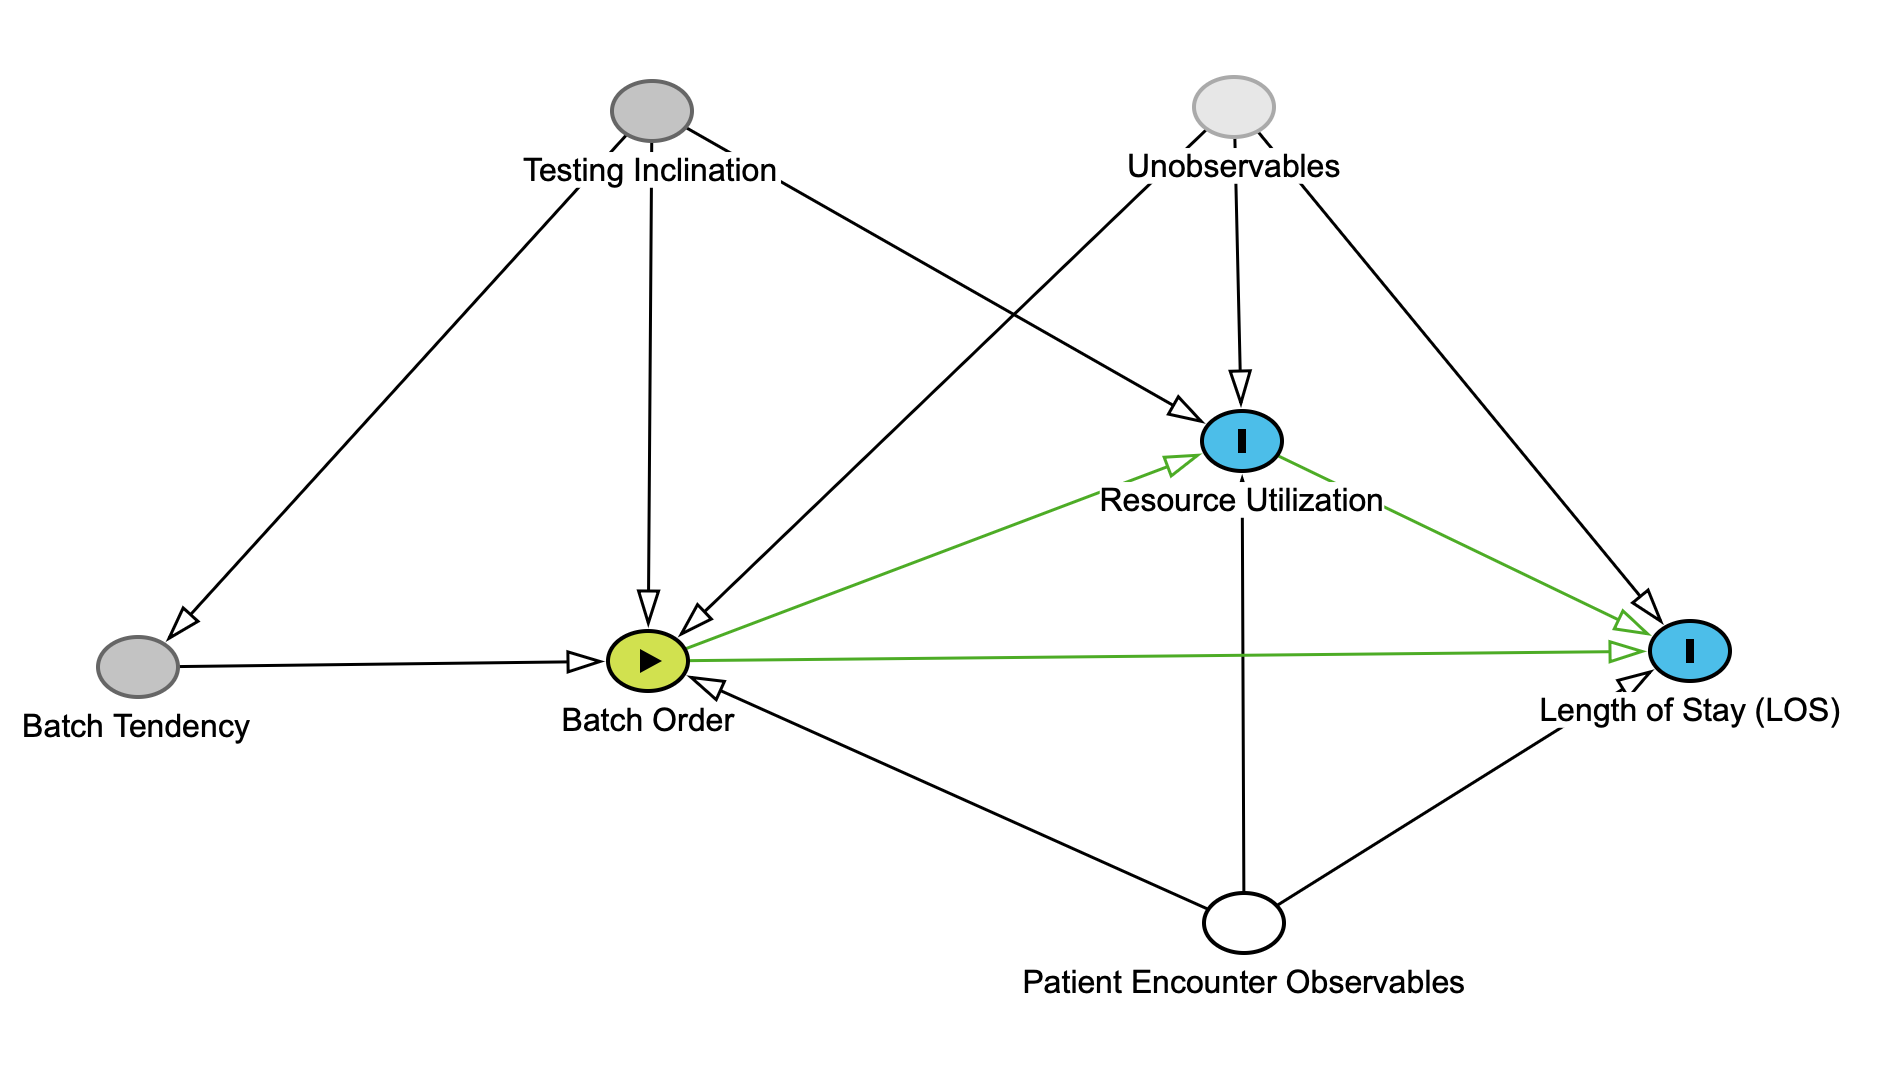
\includegraphics[width=6in]{../outputs/figures/dagitty.png}
\begin{tablenotes}
\small
\item \textit{}
\end{tablenotes}  
\end{figure}

To determine whether or not the effect of batch tendency on LOS is
mediated by the number of tests ordered, we estimate a mediation
analysis using the approach outlined by \citet{imai2010general}. Our
analysis, scrutinizes the pathways through which physician batch
tendency influences patient length of stay (LOS) in the emergency
department. The analysis delineates both direct effects, which capture
the influence of batch tendency on LOS without intermediaries, and
indirect effects, which operate through the mediator of test ordering
volume. Our findings underscore a significant Average Direct Effect
(ADE) of batch tendency on LOS, estimated at -0.15 (p = 0.046).

\hypertarget{placebo-check}{%
\subsection{Placebo Check}\label{placebo-check}}

In this section we investigate whether the reduced-form effects observed
in Section 4.1 are due to differences in batch rates across providers or
due to other provider differences correlated with batch tendency. We
start by studying reduced-form effects among patients with complaints
that are never batched, as a ``placebo/falsification check.'' By way of
example, consider a patient who arrives at the ED with a urinary tact
infection---a condition for which patients rarely undergo imaging
testing. For such patients, we should expect to see no impact of batch
tendency only if high batching and low batching physicians do not
systematically differ in other dimensions of care relevant to patient
outcomes. Conversely, if we do find a reduced-form effect for these
patients, then high batch tendency physicians must systematically differ
from low batch tendency physicians in other dimensions of care, beyond
batching.

To that end, we restrict attention to ED visits for complaints where
batching occurs no more than 10 percent of the time (recall that our
baseline sample only includes complaints with a \textgreater10 percent
batching rate). We estimate a reduced-form regression of each main
outcome on physician batch tendency for the subsample, following
equation (3). The results of this exercise are displayed in Table
\ref{tab:placebo_check}. They show that in contrast to results for our
main sample, the association between physician tendency to batch and a
given outcome is statistically indistinguishable from zero and much
smaller in magnitude for the samples of patients who visit the ED with
health conditions that are rarely batched.

\begin{table}[htbp]
\centering
\caption{Placebo Exercise: Reduced-Form Results for Rarely Batched Samples}
\label{tab:placebo_check}
\begin{tabular}{p{8cm}ccc}
\toprule
& ln(LOS) & Number of Tests & 72 Hour Return \\ 
& (1) & (2) & (3) \\
\midrule
Batch Tendency & $-0.465$ & $-0.699$ & $-0.011$ \\
& $(0.645)$ & $(0.427)$ & $(0.095)$ \\
                    &     &     &  \\
Seasonality and shift fixed effects? & Yes & Yes & Yes \\
Chief Complaint? & Yes & Yes & Yes \\
Testing inclination? & Yes & Yes & Yes \\
                    &     &     &  \\
N & 2,361 & 2,361 & 2,361 \\
\addlinespace
\midrule
\bottomrule
\end{tabular}
\begin{tablenotes}
\small
\item \textit{This table reports the estimated coefficients of a reduced-form regression of our main outcomes on physician batching tendency for samples based on the patient’s chief complaint field. Estimates come from regression on conditions that are batched less than 10 percent of the time. See text for residualization fixed effects and baseline controls. Robust standard errors are clustered at the physician level.}
\item $*** p < 0.001$, $** p < 0.01$, $* p < 0.05$.
\end{tablenotes}
\end{table}

\hypertarget{instrumental-variables-results}{%
\subsection{Instrumental Variables
Results}\label{instrumental-variables-results}}

In this section we examine the causal effects of batch ordering in the
ED. Mirroring our presentation of the reduced-form results, we turn to
presenting effects in Table \ref{tab:2SLS} on our main outcomes of ED
LOS and number of tests ordered. We first start by estimating the
effects of batch ordering on the number of tests ordered using the
standard 2SLS approach. Next we estimate the direct and indirect effects
of batch ordering on LOS using a causal mediation analysis.

\begin{table}[!htbp]
\centering
\begin{threeparttable}
\caption{Combined 2SLS and Causal Mediation Analysis Results}
\label{tab:combined_results}
\begin{tabular*}{\textwidth}{@{\extracolsep{\fill}} lcc}
\toprule
& \multicolumn{2}{c}{2SLS Results} \\
\cmidrule{2-3}
& ln(LOS) & Number of Tests \\
\midrule
Batch & -0.086 & 0.135$^{***}$ \\
& (0.419) & (0.046) \\
& & \\
\addlinespace
Seasonality and Shift Fixed Effects & Yes & Yes \\
Chief Complaint and Severity & Yes & Yes \\
\midrule
Observations & 41,901 & 41,901 \\
R$^{2}$ & 0.183 & 0.310 \\
\bottomrule
\end{tabular*}

\smallskip % Adds some space before the next part of the table

\begin{tabular*}{\textwidth}{@{\extracolsep{\fill}} lcc}
\toprule
& \multicolumn{2}{c}{Causal Mediation Analysis} \\
\cmidrule{2-3}
Effect & Estimate & 95\% CI \\
\midrule
ACME & 0.036 & [-0.009, 0.08] \\
ADE & -0.136 & [-0.221, -0.04] \\
Total Effect & -0.100 & [-0.195, 0.00] \\
Proportion Mediated & -0.333 & [-2.831, 1.21] \\
\bottomrule
\end{tabular*}

\begin{tablenotes}
\small
\item The 2SLS results are based on robust standard errors clustered at the physician level, with controls for seasonality, shift fixed effects, chief complaint, and severity. The causal mediation analysis examines whether the number of tests mediates the effect of batching on length of stay, using a quasi-Bayesian confidence interval approach with 1000 simulations.
\item $^{***} p < 0.001$, $^{**} p < 0.01$, $^{*} p < 0.05$.
\end{tablenotes}
\end{threeparttable}
\end{table}

\emph{ED length of stay (LOS).}-- Our causal mediation analysis reveals
that the Average Direct Effect (ADE) of test batching on the natural log
of LOS is -0.13607, indicating that, when not considering the mediating
effect of the number of tests, batching leads to a decrease in the
expected LOS. Specifically, this translates to an approximate 12.7
percent reduction in LOS when tests are batched, all else being equal.
This result, complemented by our 2SLS estimate of -0.086, suggests that
the direct effect of batch ordering on LOS is negative. Our results also
suggest a ``washing out'' effect, where the effeciency gains from
batching are offset by the increased number of tests ordered. This is
consistent with our finding that batching increases the number of tests
ordered.

\emph{Resource Utilization.}-- The impact of batching on resource
utilization is pronounced. We observe a 0.135 increase in the number of
tests ordered due to batching, corresponding to approximately 13.5
excess tests per 100 batch orders, where excess means tests that would
not have been ordered had the physician not batched. This result is
consistent with the notion that batching leads to increased resource
utilization in the ED.

The instrumental variable analysis presented here underscores the
complexities underlying batch ordering practices in the ED. While
batching is often seen by physicians as a method to enhance efficiency,
our findings suggest that it may lead to increased resource utilization
and that the corresponding gains in patient throughput are washed out.
These insights point to the need for a more nuanced approach to test
ordering in emergency care, one that carefully weighs the benefits of
comprehensive assessment against the risks and costs of potential
over-testing.

\hypertarget{robustness}{%
\subsection{Robustness}\label{robustness}}

The 2SLS results presented in the previous sections are robust to
several alternative specifications probing the key batching definition.
Our primary definition operationalizes batching as the ordering of
multiple diagnostic tests within a 5-minute window. This approach is
grounded in standard emergency medicine practices and offers a clear
distinction between batching and non-batching behaviors. To ensure the
robustness of our findings, we performed several sensitivity analyses.

\begin{enumerate}
\def\labelenumi{(\arabic{enumi})}
\item
  Variation in the Time Window for Batching: Firstly, we varied the time
  window for what constitutes a batch. The original 5-minute window was
  extended and contracted to understand its impact on the study's
  outcomes. Specifically, we considered scenarios where a batch is
  defined as two or more tests ordered within windows of 1 minute to 10
  minutes. This range allowed us to capture a broader spectrum of
  batching behaviors and test the sensitivity of our results to
  different batching definitions.
\item
  Refinement of Batching Definition: Secondly, we refined our batching
  definition based on the sequence and timing of test orders. In the
  initial analysis, if two tests were ordered upfront and another test
  ordered later, it was counted as a batch. We modified this definition
  to consider a set of tests as a batch only if all tests ordered during
  a patient encounter came from that initial batch order. This
  adjustment ensures that our batching definition more accurately
  reflects a comprehensive diagnostic effort at the outset of patient
  care, rather than incremental decision-making.
\end{enumerate}

The key finding from these robustness checks is the consistent impact of
batching on key outcomes across all variations. As seen in Table
\ref{tab:robustness_batching} and \ref{tab:robustness_batching2},
altering the time window for batching, whether narrowing it to as little
as 1 minute or expanding it to 10 minutes, did not qualitatively change
the results. Similarly, refining the definition of batching to consider
only those tests ordered in the initial batch also had negligible impact
on the study's main findings. These results lend further credibility to
our initial findings, demonstrating that our conclusions about the
impact of batching on patient outcomes in the ED are not sensitive to
the specific operational definition of batching.

\hypertarget{conclusion}{%
\section{Conclusion}\label{conclusion}}

Our results highlight that changes in resource utilization and costs can
arise as a consequence of small variations in physician test ordering
strategies in a single medical encounter, at the emergency department.
Our instrumental variable approach suggests that the causal effects of
batching are substantial: 13.5 excess tests arise per 100 batched
orders. This is particularly pronounced in high-volume complaint areas,
where batching leads to a significant increase in the number of tests
ordered. However, we find no significant impact of batching on ED length
of stay. Causal mediation analysis reveals that the direct effect of
batching on length of stay is negative, but this effect is offset by the
increased number of tests ordered. This suggests that the efficiency
gains from batching are washed out by the increased resource
utilization.

Our findings have important implications for emergency care practice.
While batching is often seen as a method to enhance efficiency, our
results suggest that it may lead to increased resource utilization and
that the corresponding gains in patient throughput are washed out. These
insights point to the need for a more nuanced approach to test ordering
in emergency care, one that carefully weighs the benefits of
comprehensive assessment against the risks and costs of potential
over-testing. Future research should explore the impact of batching on
other outcomes, such as patient satisfaction and clinical outcomes, to
provide a more comprehensive understanding of the implications of
batching in the emergency department.

\clearpage

\begin{APPENDIX}{General appendix}

\begin{longtable}{|p{5cm}|p{12cm}|}
\caption{Chief Complaints} \\
\hline
\textbf{Complaint Area} & \textbf{Complaints} \\
\hline
Abdominal Complaints & Abdominal Cramping, Abdominal Distention, Dyspepsia, Abdominal Pain, Ascites, Hernia, Abdominal Aortic Aneurysm, Abdominal Injury, Pancreatitis, Umbilical Hernia \\
\hline
Abnormal Test Results & Abnormal Lab, Abnormal Potassium, Abnormal Calcium, ECG Changes, Abnormal ECG, Abnormal Test Result, Blood Infection, Acute Renal Failure, Hypocalcemia, Chronic Renal Failure, Pulmonary Embolism, Abnormal X-ray, Hypoglycemic Unawareness, Elevated Blood Pressure, Abnormal Sodium, Hyperglycemia, Hyponatremia, Platelet Disorders, Anemia, Hypoglycemia, Hypertension, Hypotension, Abnormal Chest Imaging, Abnormal Oximetry, Abnormal Stress Test, Blood Sugar Problem, Hypocalcemia, Hyponatremia \\
\hline
Allergic Reaction & Allergic Reaction, Anaphylaxis \\
\hline
Back or Flank Pain & Back Pain, Back Problem, Flank Pain, Sciatica, Back Injury, Disc Disorder \\
\hline
Breast Complaints & Breast Mass, Breast Pain, Breast Problem, Breast Discharge, Breast Cancer, Breast Discharge, Breast Inflammation \\
\hline
Cardiac Arrhythmias & Atrial Fibrillation, Atrial Flutter, Cardiac Valve Problem, Bradycardia, Irregular Heart Beat, Palpitations, POTS, Ventricular Tachycardia, Rapid Heart Rate, Heart Problem, Cardiac Arrest, Congestive Heart Failure, Circulatory Problem, Transient Ischemic Attack, Ventricular Tachycardia \\
\hline
Chest Pain & Chest Injury, Chest Pain, Chest Wall Pain, Angina, Collarbone Injury, Rib Injury, Heart Pain \\
\hline
Dizziness / Lightheadedness / Syncope & Dizziness, Near Syncope, Syncope, Vertigo, Spells, Hypotension, Paroxysmal Positional Vertigo, Paroxysmal Positional Vertig \\
\hline
Ear Complaints & Cerumen Impaction, Ear Drainage, Ear Fullness, Ear Laceration, Ear Problem, Earache, Hearing Problem, Tinnitus, Ear Injury, Hearing Loss, Nasal Trauma \\
\hline
Epistaxis & Epistaxis, Epistaxis (Nose Bleed), Nose Problem \\
\hline
Exposures, Bites, and Envenomations & Animal Bite, Body Fluid Exposure, Chemical Exposure, Poisoning, Exposure to STD, Insect Bite, Smoke Inhalation, Radiation, Snake Bite, Toxic Inhalation \\
\hline
Extremity Complaints & Ankle Injury, Ankle Pain, Arm Injury, Arm Pain, Cold Extremity, Arm Swelling, Arthritis, Elbow Injury, Elbow Pain, Pseudogout, Extremity Pain, Extremity Weakness, Finger Injury, Hip Injury, Extremity Weakness, Finger Injury, Finger Pain, Dislocation, Foot Infection, Foot Injury, Foot Numbness, Foot Pain, Foot Swelling, Foot Ulcer, Foot Wound Check, Hand Injury, Hand Pain \\
\hline
Eye Complaints & Blurred Vision, Decreased Visual Acuity, Diplopia, Detached Retina, Eye Drainage, Eye Exposure, Eye Pain, Eye Problem, Eye Swelling, Eye Trauma, Foreign Body Eye, Flashes / Light, Loss of Vision, Red Eye, Visual Field Change, Eyelid Problem, Itchy Eye, Eye Exam, Burning Eyes, Eye Twitching, Eyelid/brow Lift Evaluation, Strabismus, Glaucoma, Spots / Floaters \\
\hline
Falls, Motor Vehicle Crashes, Assaults, and Trauma & Assault Victim, Concussion, Facial Injury, Fall, Nasal Trauma, Head Injury, Head Laceration, Motor Vehicle Crash, Puncture Wound, Sexual Assault, Trauma, Domestic Violence, Gun Shot Wound, Work Related Injury, Motorcycle Crash, Injury, Bicycle Accident, Near Drowning, Lip Laceration \\
\hline
Fatigue and Weakness & Difficulty Walking, Fatigue, Gait Problem, Weakness-Generalized, Chronic Fatique, Weakness- Generalized \\
\hline
Fevers, Sweats or Chills & Chills, Diaphoresis, Fever, Night Sweats, Diaphoretic, Diapohresis, Hoarseness, Laryngitis \\
\hline
Foreign Body & Food Bolus, Foreign Body, Foreign Body in Ear, Foreign Body in Skin, Foreign Body in Vagina, Swallowed Foreign Body, Foreign Body in Nose, Foreign Body, FB eye, Foreign Body in Rectum \\
\hline
Gastrointestinal Issues & Anal Fissure, Black or Bloody Stool, Constipation, GERD, Anal Fistula, Diarrhea, Dysphagia, Fecal Impaction, Fistula Follow Up, GIbleeding, GI Problem, Hemorrhoids, Morning Sickness, Nausea, Ostomy Care, Rectal Bleeding, Rectal Pain, Vomiting, Vomiting Blood, Vomiting During Pregnancy, GI Bleeding, Fecal Incontinence, Bloated, Hematochezia, Urine Leakage, Heartburn, Rectal Discharge, Urolithiasis, Ulcerative Colitis, Irritable Bowel Syndrome, Rectal Prolapse, Fistula Evaluation, Rectal Problems, Perianal Abscess, Fisula Evaluation, Stoma Dysfunction \\
\hline
Genital Complaints & Groin Burn, Groin Pain, Groin Swelling, Inguinal Hernia, Menstrual Problem, Pelvic Pain, Penis Pain, Priapism, Testicle Pain, Menorrhagia, Vaginal Bleed, Vaginal Bleeding, Vaginal Itching, Bartholin's Cyst, Genital Warts, Groin Injury, Vaginal Bleeding-Pregnant, Vag Bleed Pregnant, Female Genital Issue, Penis Injury, Vaginal Discharge, Vaginal Pain, Erectile Dysfunction, Vaginal Prolapse, Urethral Stricture, Penile Discharge, Menorrhagia, Gynecologic Exam, Menstrual Problem, Vaginitis/Bacterial Vaginosis, Ovarian Cyst, Vaginitis / Bacterial Vaginosi \\
\hline
Medical Device or Treatment Issue & Cast Problem, Device Check, Dressing Change, Feeding Tube, AICD Problem, Insulin Pump Visit, Gastrostomy Tube Change, Medication Reaction, Shunt, Appliance Removal, Tube Problem, Urinary Catheter Change, Vascular Access Problem, Enteral Nutrition Evaluation, Device Malfunction, Pacemaker Problem, Remova /  Exchange Catheter, Drain Removal, Outpatient Infusion, Treatment, Heart Assist Device, Stoma Dysfunction, Tracheostomy Tube Change, Ureteral Stent Exchange \\
\hline
Medication Request & Immunizations, Infusion / Injection Administration, IV Medication, Infusion/ Injection Administ, Med Refill, Medication Visit, Pain Management, Blood Product Administration, Labs Only, Tetanus (Td \& Tdap), Wound Care \\
\hline
Neurological Issue & Altered Mental Status, Cognitive Concerns, Facial Droop, Pre Syncope, Focal Weakness, Headache, Memory Loss, Migraine, Dementia, Dysphasia, Neuro Problem, Numbness, Paralysis, Seizures, Slurred Speech, Spasms, Stroke Like Symptoms, Tingling, Tremors, Trigeminal Neuralgia, Unable to Speak, Seizure Disorder, Insomnia, Parkinson's Disease, Loss of Consciousness, Neuropathy, Ataxia, Unable to speak, Peripheral Neuropathy, Stroke, Cerebrovascular Accident, Speech Problem, Acute Neurological Problem, Flashes, Light, Unresponsive, Multiple Sclerosis, Parkinson's Disease, Febrile Seizure, Paresthesia, Peripheral Neuropathy, Hydrocephalus, Spasticity, Neuroendocrine Tumor \\
\hline
Other & Dehydration, Fisula Evaluation, Follow-Up, Illness, Letter for School/Work, Aneurysm, Lung Eval, Error, Mass, Oral Swelling, Other, Advice Only, Deformity, Electric Shock, Personal Problem, Shaking, Swelling, Swollen Glands, Adenopathy, Adrenal Problem, Thrombophilia, Weight Gain, Weight Loss, Hiccups, , Chemo Related Symptoms, Hot Flashes, Follow-up, Non Healing Wound, (Other), Mouth Injury, Xerostomia, Prostate Check, Suture / Staple Removal, Wellness, Voice Changes, Vital Sign Check, Coagulation Disorder, Cold Exposure, Consult, Dental Problem, Tetanus (Td \& Tdap), Infusion/ Injection Administ, Tracheostomy Tube Change, Medical Information, Neutropenic Fever, Infection, Leukemia, Heat Exposure, Poor Appetite, Gingivitis, Pre-op Exam, gingivitis, Loss of appetite, Failure To Thrive, Referral, Lymphoma, Hot Flashes, Neutropenia, Radiation, Ingestion, TB Test, Fussy, Lupus, Toxic Inhalation, Lung Screening, Leakage/Loss of Fluid, Liver Eval, Hepatic Cancer, Lung Mass, Venous Thromboembolic Disease, Insulin Pump Visit, Preventive Visit, Avulsion, Peripheral Edema, Hypoglycemic Unawareness, Immobility, Giant Cell Arteritis, Polydipsia, Platelet Disorders, Post-procedure, Lung Follow-up, Poisoning, Injections, POTS, Insulin Reaction, Liver Transplant, Labs Only \\
\hline
Other Pain & Dental Pain, Facial Pain, Generalized Body Aches, Myalgia, Dental Injury, Jaw Pain, Muscle Pain, Neck Pain, Pain, Sickle Cell Pain Crisis, Paresthesia, Torticollis, Chronic Pain, Cancer Pain, Incisional Pain, Bone Pain, Tailbone Pain, Gout, Muscle pain/Weakness, Pseudogout \\
\hline
Post-Op Issue & Post-Op, Post-Procedure, Post-Op Problem, Post-op, Post-Op Issue, Wound Dehiscence, Post-op Problems, Post-op Problem \\
\hline
Psychiatric Complaints & Anxiety, Auditory Hallucinations, Depression, Panic Attack, Homicidal, PTSD (Post-Traumatic Stress, Delusional, Fussy, Paranoia, Suicide Attempt, Hallucinations, Manic Behavior, Eating Disorder, Suicidal, Agitation, Psychiatric Evaluation, Aggressive Behavior, Mental Health Problem, Inappropriate Words \\
\hline
Shortness of Breath & Airway Obstruction, Aspiration, Pain With Breathing, Near Drowning, Respiratory Distress, Shortness of Breath, Wheezing, Increased Work Of Breathing, Difficulty Breathing, Choking, Oxygen Dependence, Hyperventilating, Orthopnea \\
\hline
Skin Complaints & Abrasion, Abscess, Bleeding/Bruising, Blister, Angioedema, Lip Laceration, Burn, Cellulitis, Cyst, Drainage from Incision, Disturb of Skin Sens, Edema, Extremity Laceration, Facial Burn, Cyanosis, Impetigo, Facial Laceration, Facial Swelling, Finger Laceration, Leg Rash, Herpes Zoster, Hives, Itching, Jaundice, Diabetic Ulcer, Diabetic Wound, Laceration, Mouth Lesions, Non-Healing Wound, Rash, Recurrent Skin Infections, Skin Problem, Sore, Scabies, Suture \textbackslash Staple Removal, Wound Check, Wound Infection, Lesion, Skin Check, Minor Skin Infection, Skin Ulcer, Skin Discoloration, Sunburn, Head Lice, Scabies, Fungal Infection, Leg Rash, Impetigo \\
\hline
Substance Abuse Issues & Alcohol Intoxication, Alcohol Problem, Withdrawal, Drug Overdose, Drug / Alcohol Dependency, Addiction Problem, Addiction Assessment, Delirium Tremens (DTS) \\
\hline
Upper Respiratory Symptoms & Congestion, Cough, Coughing Up Blood, Flu Symptoms, Enlarged Tonsils, Peritonsillar Abscess, Nasal Congestion, Sinus Symptoms, Sinusitis, Sore Throat, Hoarseness, Throat Problem, Upper Respiratory Infection, Influenza, Laryngitis, Respiratory Arrest, Pneumonia, Pleural Effusion, Asthma, Croup, URI, Peritonsillar Abscess \\
\hline
Pregnancy Related & Pregnancy Problem, Miscarriage, Contractions, Ectopic Pregnancy, Laboring, Possible Pregnancy, Pregnancy Related \\
\hline
Renal & Av Fistula, Kidney Transplant, Elevated Serum Creatinine, End-Stage Liver Disease, Hemodialysis Access, Nephritis, Ureteral Stent Exchange \\
\hline
Urinary Complaints & Bladder Problem, Blood in Urine, Cystitis, Difficulty Urinating, Dysuria, Gross Hematuria, Painful Urination, Urinary Frequency, Urinary Symptom, Urinary Incontinence, Urinary Problem, Urinary Retention, Slowing Urinary Stream, Urinary Tract Infection, Urinary Urgency, Voiding Dysfunction, Hesitancy Urinary \\
\hline
\end{longtable}

\newpage

\begin{table}[!htbp]
\centering 
  \caption{Testing the Monotonicity Assumption} 
\label{tab:monotonicity}
\begin{tabular}{@{\extracolsep{5.5pt}}lcc} 
\\[-1.8ex]\hline 
\hline \\[-1.8ex] 
Sub-sample margin & Baseline Tendency  & Reverse-Sample Tendency \\ 
\hline \\[-1.8ex] 
Extremity Complaints & 0.864$^{***}$ (0.128) & 0.893$^{***}$ (0.068) \\ 
Upper Respiratory Symptoms & 1.235$^{***}$ (0.247) & 0.953$^{***}$ (0.038) \\ 
Abnormal Test Results & 0.980$^{***}$ (0.219) & 0.766$^{***}$ (0.111) \\
Falls, Motor Vehicle Crashes, Assaults, and Trauma & 1.061$^{***}$ (0.167) & 0.784$^{***}$ (0.103) \\
Shortness of Breath & 1.204$^{***}$ (0.232) & 0.944$^{***}$ (0.047) \\
Gastrointestinal Issues & 1.049$^{***}$ (0.140) & 0.929$^{***}$ (0.052) \\
Chest Pain & 1.073$^{***}$ (0.223) & 0.943$^{***}$ (0.048) \\
Dizziness/Lightheadedness/Syncope & 1.899$^{***}$ (0.171) & 0.930$^{***}$ (0.042) \\
Back or Flank Pain & 0.657$^{***}$ (0.180) & 0.718$^{***}$ (0.106) \\
Neurological Issue & 0.970$^{***}$ (0.191) & 0.835$^{***}$ (0.067) \\
Fatigue and Weakness & 1.698$^{***}$ (0.230) & 0.938$^{***}$ (0.058) \\
Cardiac Arrhythmias & 2.571$^{***}$ (0.243) & 1.107$^{***}$ (0.059) \\
Abdominal Complaints & 0.903$^{***}$ (0.275) & 0.971$^{***}$ (0.019) \\
Skin Complaints & 0.448$^{***}$ (0.098) & 0.584$^{***}$ (0.108) \\
Fevers, Sweats or Chills & 1.033$^{***}$ (0.305) & 0.888$^{***}$ (0.084) \\
\hline \\[-1.8ex] 
\end{tabular} 
\begin{tablenotes}
\small
\item \textit{Column 1 displays the first stage coefficient of batched on the baseline physician batch tendency instrument for the corresponding sub-sample. Column 2 constructs a new physician batch tendency instrument using all emergency visits, excluding the corresponding sub-sample (``reverse-sample"), and displays the coefficient of the first stage regression back on that sub-sample. Robust standard errors are clustered at the physician level.}
\item $*** p < 0.001$, $** p < 0.01$, $* p < 0.05$.
\end{tablenotes}
\end{table}

\newpage

\begin{table}[!htbp] \centering 
  \caption{2SLS Results: Robustness to Batching Definition (1-minute and 10-minute windows)} 
  \label{tab:robustness_batching} 

\begin{tabular}{@{\extracolsep{10pt}}lccc} 
\\[-1.8ex]\hline 
\hline \\[-1.8ex] 
 & \multicolumn{3}{c}{\textbf{1-minute window}} \\
\\[-1.8ex] & Log LOS & Number of Tests & 72 Hour Return \\ 
\\[-1.8ex] & (1) & (2) & (3)\\ 
\hline \\[-1.8ex] 
 Testing Inclination & 0.592$^{***}$ & 0.975$^{***}$ & $-$0.025$^{***}$ \\ 
  & (0.203) & (0.018) & (0.009) \\ 
  & & & \\ 
 Batch & $-$0.101 & 0.159$^{***}$ & 0.021 \\ 
  & (0.496) & (0.054) & (0.023) \\ 
  & & & \\ 
\textit{N} & 41,929 & 41,929 & 41,929 \\ 
R$^{2}$ & 0.209 & 0.278 & 0.009 \\ 
Adjusted R$^{2}$ & 0.204 & 0.274 & 0.003 \\ 
Residual Std. Error & 0.492 & 0.836 & 0.184 \\ 
\hline 
\\[-1.8ex] & \multicolumn{3}{c}{\textbf{10-minute window}} \\
\\[-1.8ex] & Log LOS & Number of Tests & 72 Hour Return \\ 
\\[-1.8ex] & (1) & (2) & (3)\\ 
\hline \\[-1.8ex] 
 Testing Inclination & 0.650$^{***}$ & 0.957$^{***}$ & $-$0.027$^{**}$ \\ 
  & (0.241) & (0.022) & (0.011) \\ 
  & & & \\ 
 Batch & $-$0.205 & 0.141$^{***}$ & 0.017 \\ 
  & (0.438) & (0.045) & (0.018) \\ 
  & & & \\ 
\textit{N} & 41,929 & 41,929 & 41,929 \\ 
R$^{2}$ & 0.146 & 0.315 & 0.009 \\ 
Adjusted R$^{2}$ & 0.141 & 0.311 & 0.003 \\ 
Residual Std. Error & 0.512 & 0.814 & 0.184 \\ 
\hline 
\hline \\[-1.8ex] 
\end{tabular}
\begin{tablenotes}
\small
\item $*** p < 0.001$, $** p < 0.01$, $* p < 0.05$.
\end{tablenotes}
\end{table}

\newpage

\begin{table}[!htbp] \centering 
  \caption{2SLS Results: Robustness to Batching Definition (all tests at once)} 
  \label{tab:robustness_batching2} 
  
\begin{tabular}{@{\extracolsep{5pt}}lccc} 
\\[-1.8ex]\hline 
\hline \\[-1.8ex] 
\\[-1.8ex] & Log LOS & Number of Tests & 72 Hour Return \\ 
\\[-1.8ex] & (1) & (2) & (3)\\ 
\hline \\[-1.8ex] 
 Batch & 0.592$^{***}$ & 0.975$^{***}$ & $-$0.025$^{***}$ \\ 
  & (0.203) & (0.018) & (0.009) \\ 
  & & & \\ 
 `any.batch(fit)` & $-$0.101 & 0.159$^{***}$ & 0.021 \\ 
  & (0.496) & (0.054) & (0.023) \\ 
  & & & \\ 
\textit{N} & 41,929 & 41,929 & 41,929 \\ 
R$^{2}$ & 0.209 & 0.278 & 0.009 \\ 
Adjusted R$^{2}$ & 0.204 & 0.274 & 0.003 \\ 
Residual Std. Error (df = 41667) & 0.492 & 0.836 & 0.184 \\ 
\hline 
\hline \\[-1.8ex] 
\textit{Notes:} & \multicolumn{3}{r}{$^{***}$Significant at the 1 percent level.} \\ 
 & \multicolumn{3}{r}{$^{**}$Significant at the 5 percent level.} \\ 
 & \multicolumn{3}{r}{$^{*}$Significant at the 10 percent level.} \\ 
\end{tabular} 
\end{table}

\newpage

\begin{table}[ht]
\centering
\caption{2SLS Results for the "Batch" Variable Across Different General Complaints: Outcome of Number of Tests}
\begin{tabular}{lcc}
\hline
\textbf{Complaint} & \textbf{Batching Coefficient} & \textbf{Standard Error} \\
\hline
Musculoskeletal/Extremity & 0.476** & (0.235)  \\
Respiratory-Related & 0.244 & (0.209)   \\
General/Other Symptoms & 0.179 & (0.207)   \\
Gastrointestinal/Abdominal & -0.092 & (0.128)   \\
Cardiac/Chest-Related & 0.270 & (0.264)   \\
Neurological/Syncope & -0.080 & (0.493)   \\
\hline
\end{tabular}
\label{tab:batch_variable_outcome}
\end{table}

\end{APPENDIX}

% Appendix here
% Options are (1) APPENDIX (with or without general title) or
%             (2) APPENDICES (if it has more than one unrelated sections)
% Outcomment the appropriate case if necessary
%
% \begin{APPENDIX}{<Title of the Appendix>}
% \end{APPENDIX}
%
%   or
%
% \begin{APPENDICES}
% \section{<Title of Section A>}
% \section{<Title of Section B>}
% etc
% \end{APPENDICES}


% Acknowledgments here
\ACKNOWLEDGMENT{The authors would like to thank ..}

\bibliographystyle{informs2014}
\bibliography{references.bib}



\end{document}
